%!TEX root = ../dissertation.tex

\chapter{Solution}
\label{chapter:solution}
This chapter proposes a solution to determine if a cloud-based deployment is able to meet the
fundamental requirements of \gls{IoT} applications. As described in Chapter \ref{chapter:introduction},
we will follow two approaches to deploy the smart warehouse application in the cloud, the cloud-based
and the fog-based approach. Furthermore, we also proposed a mechanism to automate the provisioning of
RFID applications middleware in the cloud.

% Smart Warehouse Deployment
\section{Smart Warehouse Deployment}
\label{sec:smart_warehouse_deployment}
As described in Section \ref{sub:domain}, our smart warehouse is a system composed of smart objects
that can be identified by readers and sensors that are deployed in the place. In traditional solutions,
the application is provisioned in a local infrastructure. Although such approach guarantees that
the low-latency requirements are meet, this solution comes with several bottlenecks - such as the
low scalability, infrastructure and maintenance costs - that can be a barrier for these applications.\\

Leveraging the infrastructure required to provisioning the \gls{IoT} applications to the cloud
guarantees that the bottlenecks of traditional solutions are solved. However, we also need
to guarantee that the latency requirements of these applications are fulfilled. The following sections
describes the approaches to deploy the application in the cloud and to automate their provisioning.

% Cloud approach
\subsection{Cloud Deployment}
\label{sub:sol_cloud}

% Cloud approach
\begin{figure}[ht!]
  \centering
  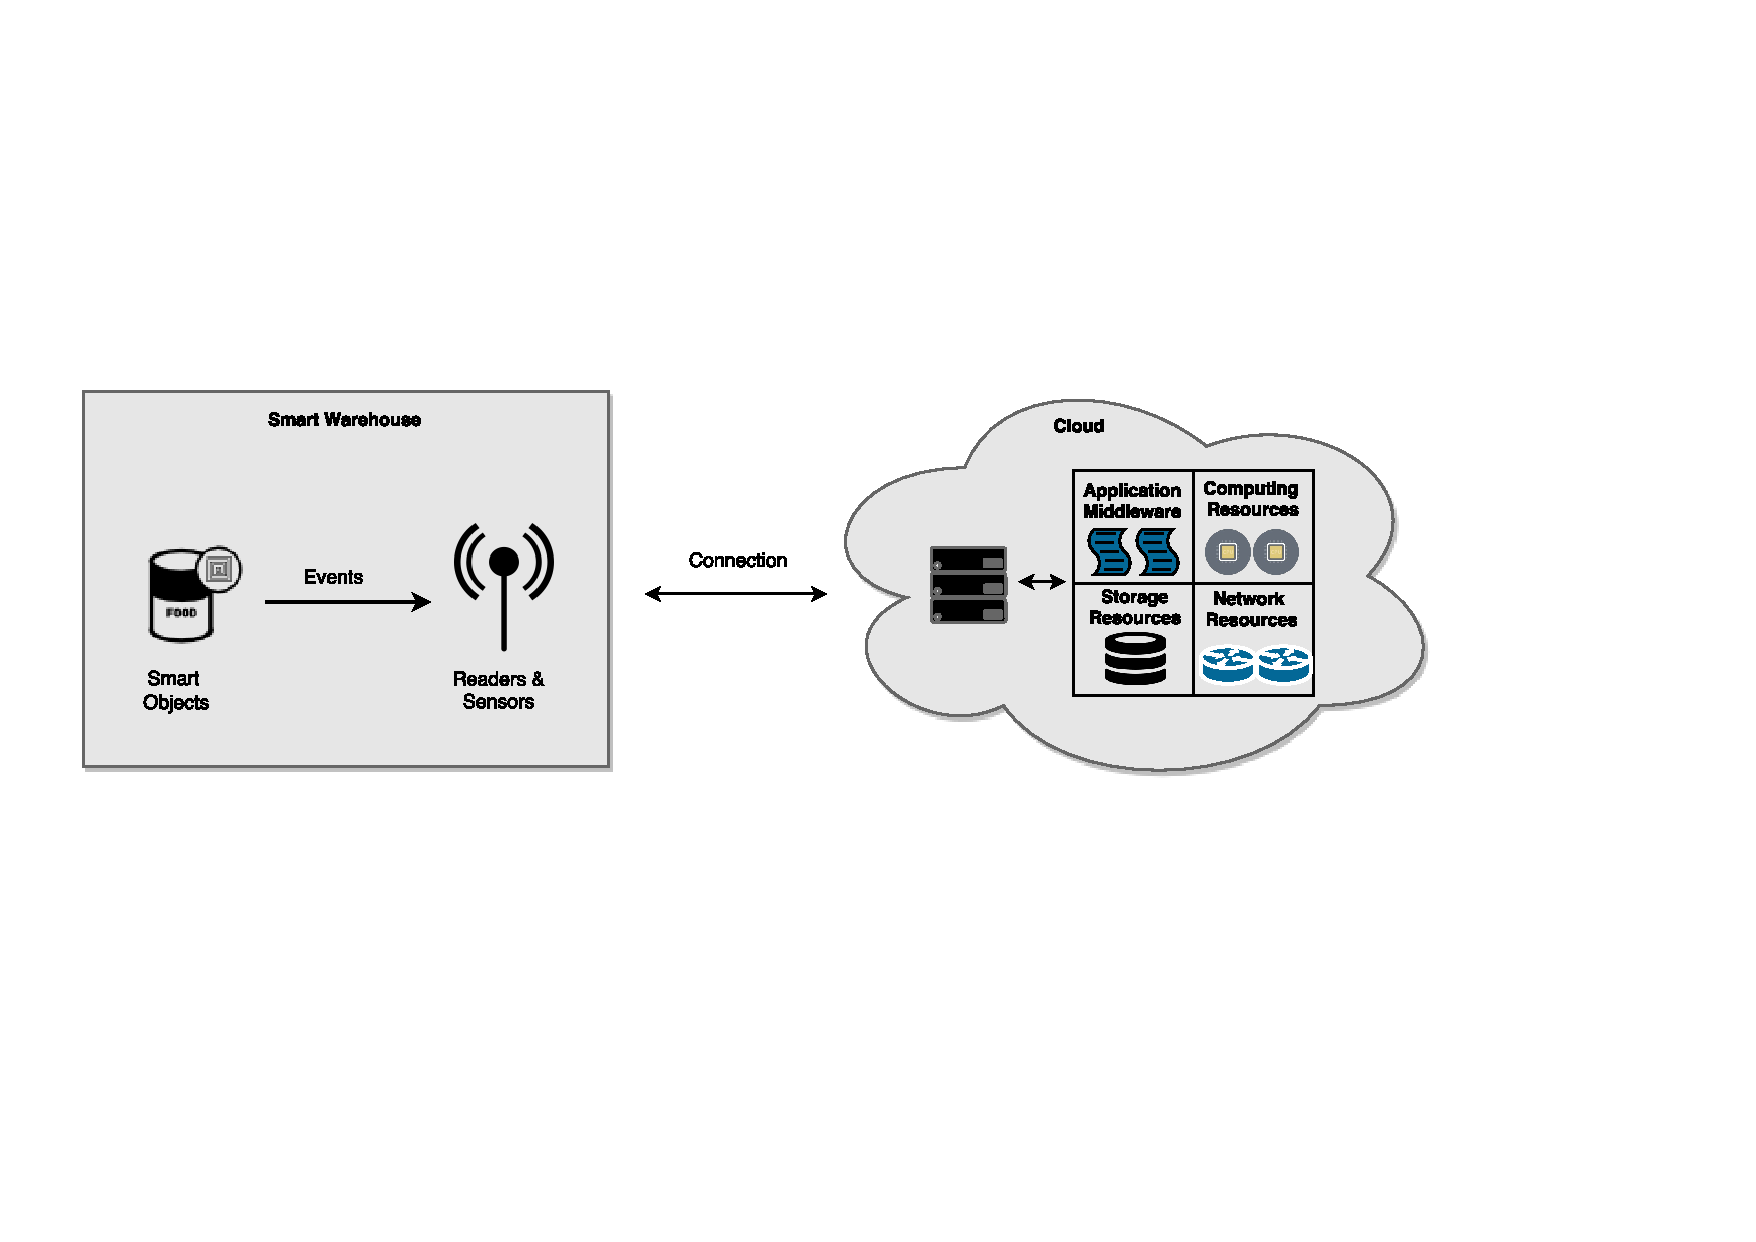
\includegraphics[width=\textwidth]{./images/solution_cloud_architecture}
  \caption{Cloud-approach: smart warehouse conceptual architecture.}
  \label{fig:solution_cloud_architecture}
\end{figure}

Figure~\ref{fig:solution_cloud_architecture} presents the architecture of a cloud-based smart warehouse.
The warehouse is composed of smart objects, sensors and readers that capture the events that occurs
in the warehouse. The application middleware is provisioned in the cloud, which virtualizes the computing,
storage and network resources needed to support the application.\\

The smart warehouse is connected to the cloud through a wireless connection such as Wi-Fi, 3G or
\gls{LTE}.

% Fog approach
\subsection{Fog Deployment}
\label{sub:sol_fog}

% Fog approach
\begin{figure}[ht!]
  \centering
  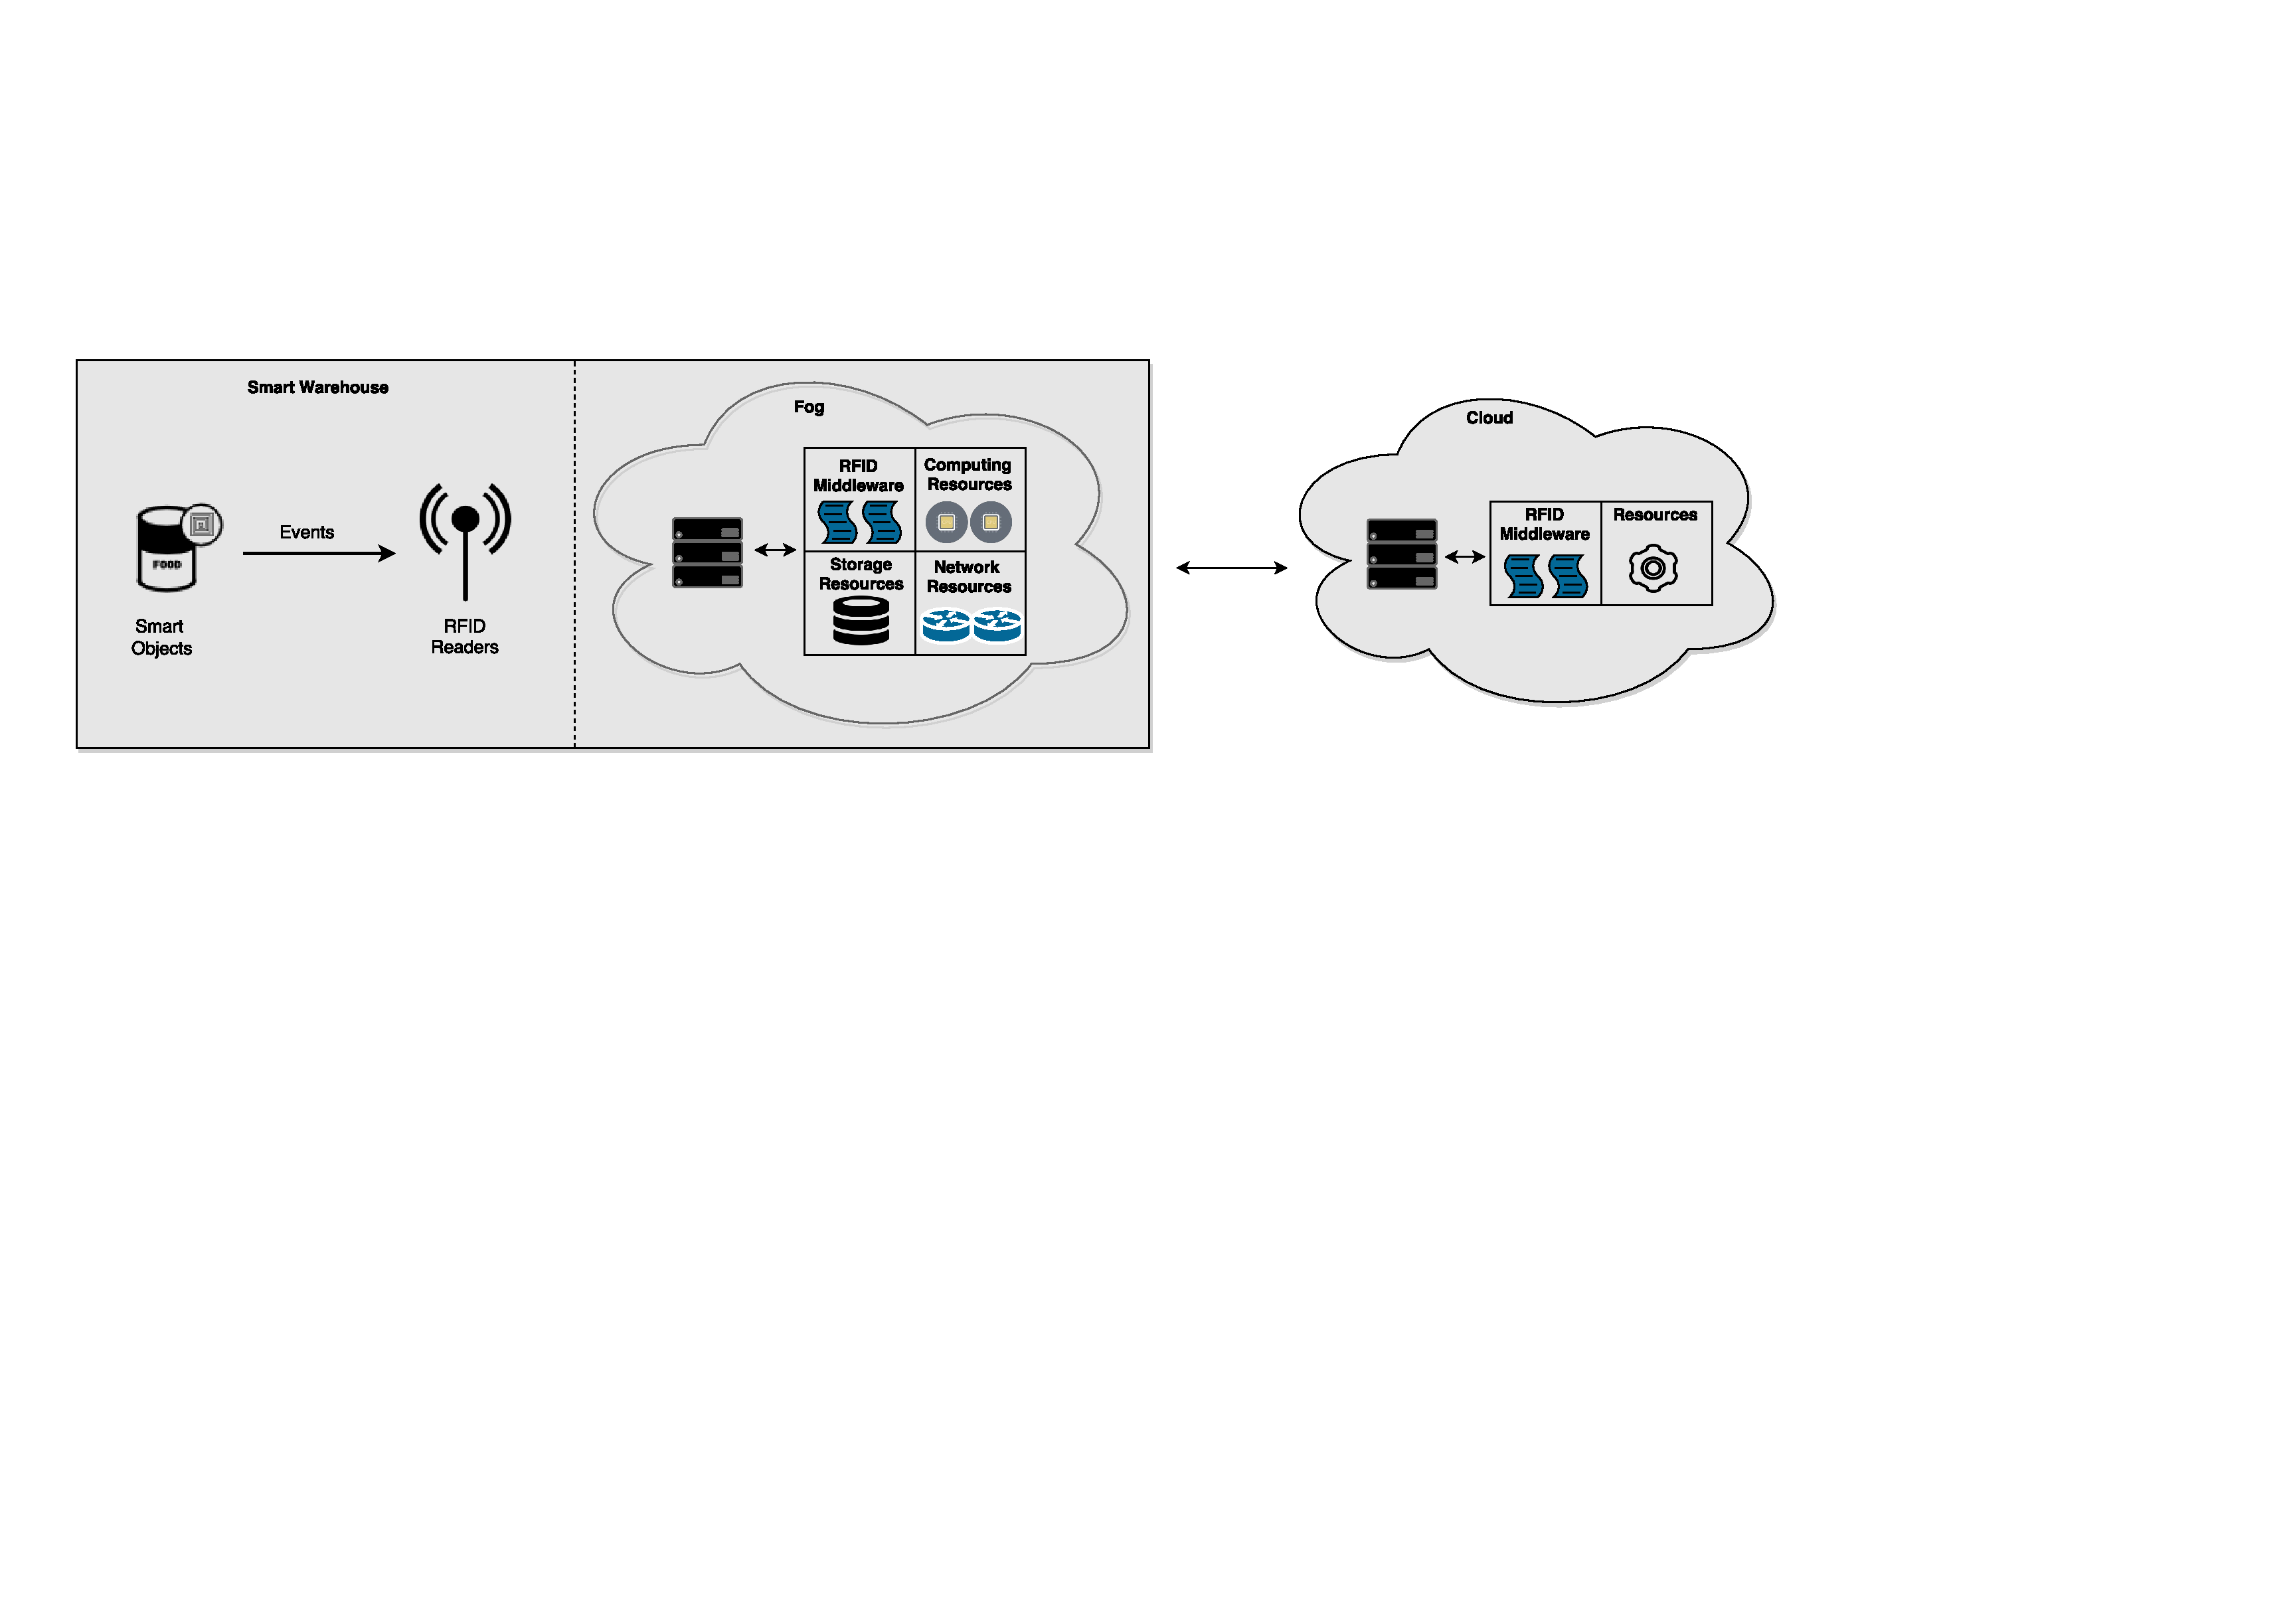
\includegraphics[width=\textwidth]{./images/solution_fog_architecture}
  \caption{Fog-approach: smart warehouse conceptual architecture.}
  \label{fig:solution_fog_architecture}
\end{figure}

Figure~\ref{fig:solution_fog_architecture} presents the architecture of a fog-based smart warehouse.
As in the cloud-based approach the warehouse is composed of smart objects, sensors and readers.
The proposed approach aims to extend the cloud paradigm to the edge of the network. The fog achieves
that by virtualizing computing, storage and network resources. Unlike the cloud infrastructure, that
usually is provisioned thousands of kilometers from the smart warehouse, the fog infrastructure
usually is provisioned closest to the smart warehouse network.\\

Regarding the application middleware, the application components are distributed across the cloud and
the fog. The components responsible to store the data during a long period of time are provisioned in
the cloud. The components responsible to perform real-time processing of the data generated in the
warehouse, and the components that filter the data that is consumed locally and must be delivered to
the cloud are provisioned in the fog.\\

The smart warehouse can be connected to the fog through several types of connection, from a physical
connection to a wireless connection such as Wi-Fi, 3G or \gls{LTE}. The fog is connected to the cloud
through a wireless connection, typically a Wi-Fi connection.

% Provisioning
\section{Provisioning}
\label{sec:provisioning}
In this section we propose a mechanism that automates the provisioning of software for \gls{IoT} applications
in the cloud. Our solution relies on configuration management tools that leverage existing software
stacks. Figure~\ref{fig:provisioning_generic_architecture} presents the architecture for the proposed
mechanism.\\

% Provisioning mechanism conceptual architecture
\begin{figure}[ht!]
  \centering
  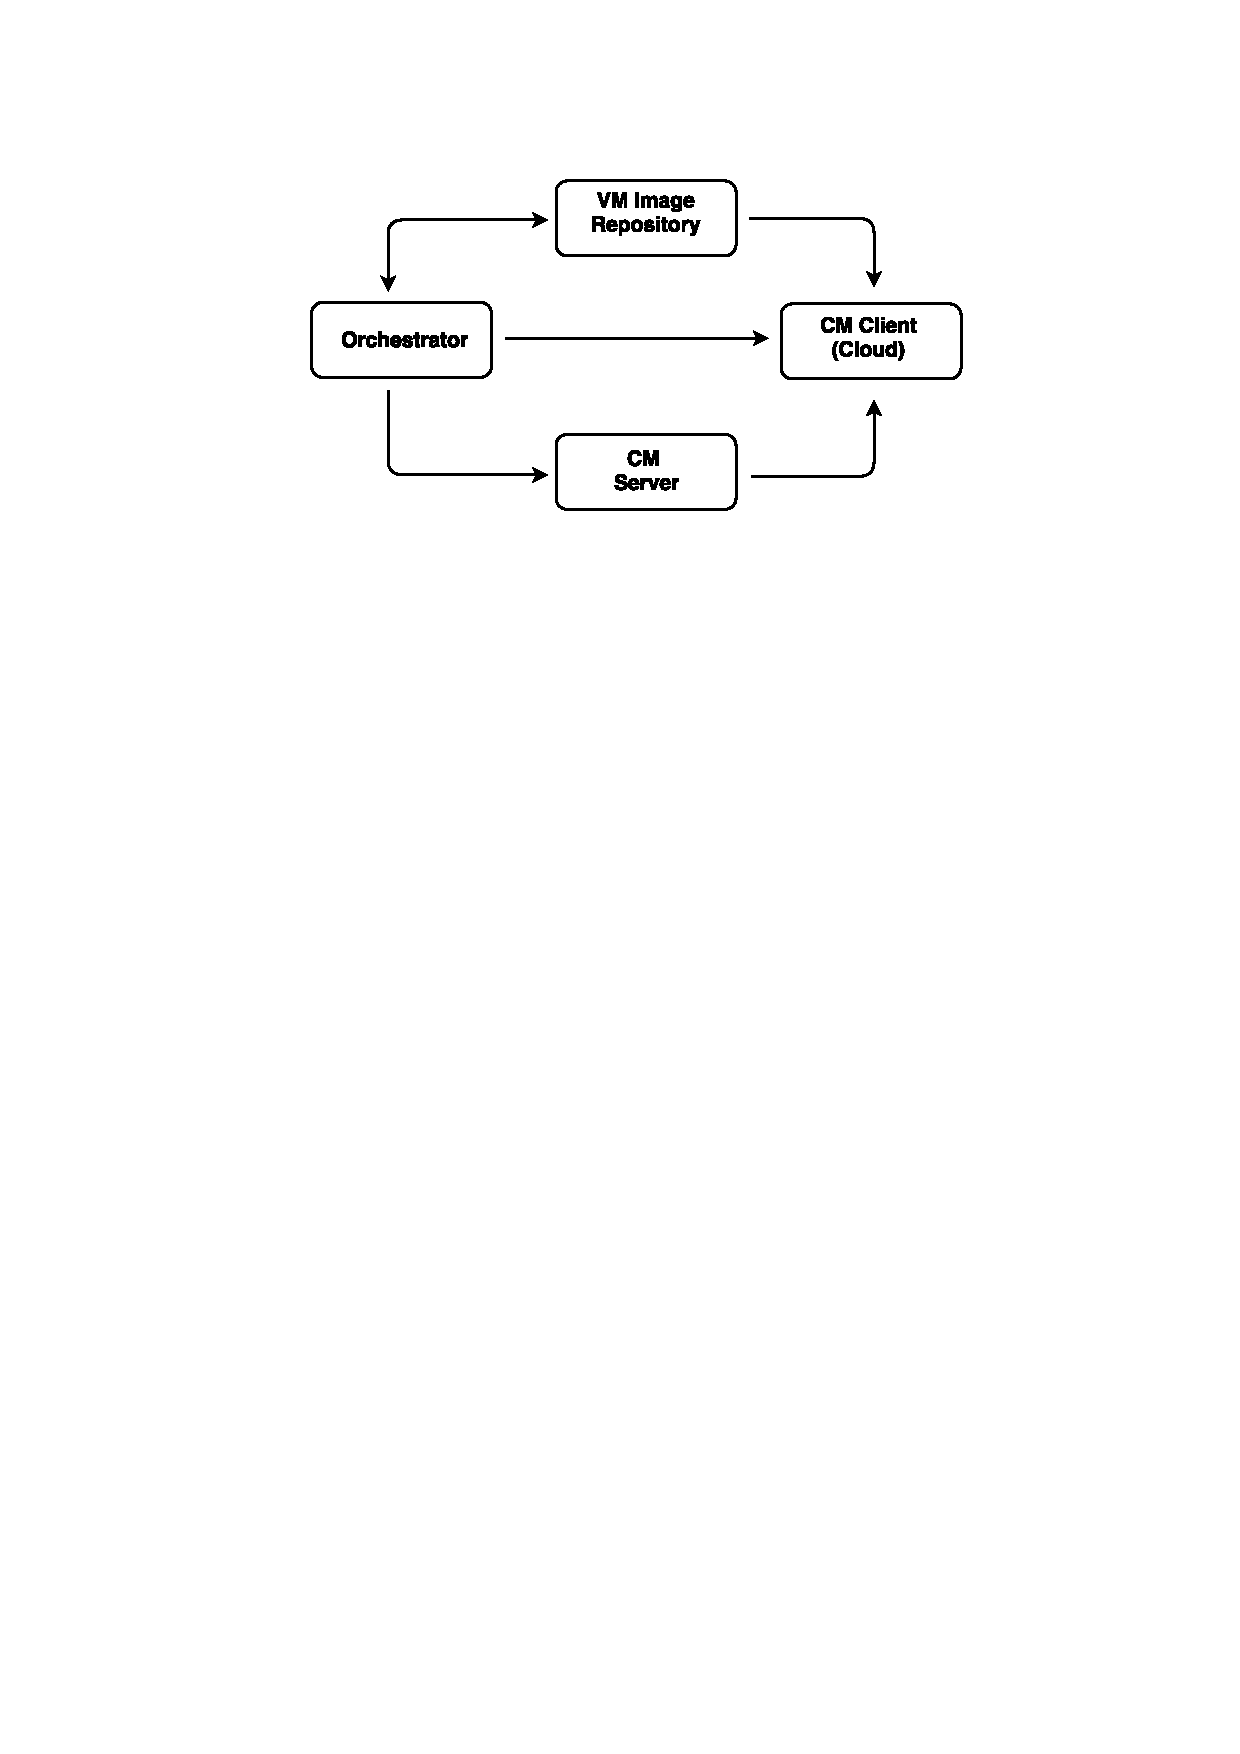
\includegraphics[width=.7\textwidth]{images/c4t-generic-solution.pdf}
  \caption{Provisioning mechanism conceptual architecture.}
  \label{fig:provisioning_generic_architecture}
\end{figure}

In the proposed architecture, the provisioning policies and software images of a smart place are
defined and configured in a local environment and then uploaded to its respective remote repositories.
When the provisioning request is performed - through a configuration management interface in the local
environment - the configuration management (CM) client in the server node pulls the polices from the
configuration management server, a centralized server that is responsible to maintain a consistent
state of the provisioned nodes in the cloud. In order to enforce the polices, the CM client pulls the
software images from a central repository and then performs the provisioning and configuration of
the software. After provisioning the infrastructure, the CM client periodically polls the CM server
in order to determine if its current state is consistent with the most recent policy.
